\documentclass[tikz,border=3.14pt]{standalone}
\usepackage{tikz}
\usetikzlibrary{arrows.meta}
\usepackage{amsmath}
\usepackage{physics}

\ExplSyntaxOn
\msg_redirect_name:nnn { siunitx } { physics-pkg } { none }
\ExplSyntaxOff

\begin{document}
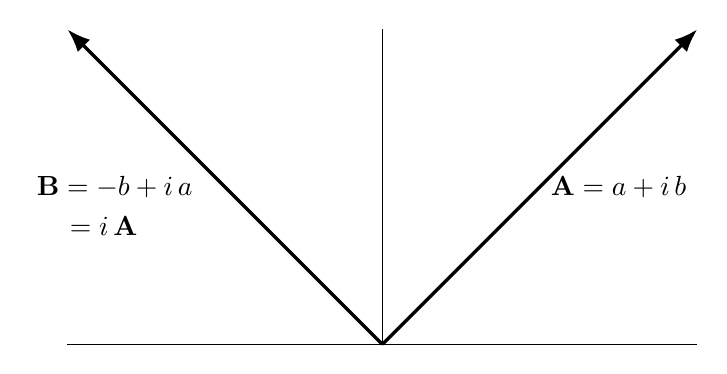
\begin{tikzpicture}[scale=2,
		vector/.style={-{Latex}, very thick}]

        \draw (-2, 0) -- (2, 0);
        \draw (0, 0) -- (0, 2);
        \draw [vector] (0, 0) -- (2, 2);
        \node at (1.5, 1) {$\vb{A} = a + i \, b$};
        \draw [vector] (0, 0) -- (-2, 2);
        \node at (-1.7, 1) {$\vb{B} = - b + i \, a$};
        \node at (-1.77, 0.75) {$= i \, \vb{A}$};

\end{tikzpicture}
\end{document}